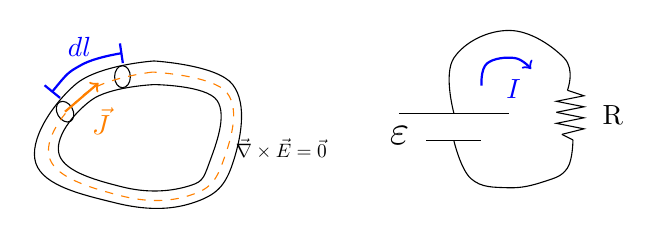
\begin{tikzpicture}
\draw  plot[smooth, tension=.7] coordinates {(-2.553,1.6209) (-3.553,1.3209) (-4.053,0.3209) (-3.053,-0.1791) (-2.053,-0.1791) (-1.553,0.3209) (-1.553,1.3209) (-2.553,1.6209)};
\draw  plot[smooth, tension=.7] coordinates {(-2.553,1.3209) (-3.353,1.1209) (-3.753,0.4209) (-2.953,0.0209) (-2.153,0.0209) (-1.853,0.3209) (-1.753,1.1209) (-2.553,1.3209)};
\draw  (-2.953,1.4209) ellipse (0.1 and 0.14);
\draw [rotate=30] (-2.7006,2.6874) node (v1) {} ellipse (0.1 and 0.14);
\draw [->, thick, orange](v1.center) -- (-3.2568,1.3409) node[midway, below right]{$\vec{J}$};
\draw  [dashed, orange]plot[smooth, tension=.7] coordinates {(-2.5695,1.4801) (-3.4402,1.1969) (-3.8767,0.3797) (-2.9897,-0.0869) (-2.1005,-0.0869) (-1.6804,0.3333) (-1.6246,1.2155) (-2.5695,1.4801)};
\draw [|-|, thick, blue] plot[smooth, tension=.7] coordinates {(-3.853,1.2209) (-3.4701,1.5734) (-2.953,1.7209)};
\node [blue] at (-3.4984,1.8046) {$dl$};
\node [scale=0.7] at (-0.9355,0.5) {$\vec{\nabla}\times\vec{E}=\vec0$};
\draw  [scale=0.7](0.7938,1.3696) -- (2.7938,1.3696);
\draw  [scale=0.7](1.2938,0.8696) -- (2.2938,0.8696);
\draw  [scale=0.7] plot[smooth, tension=.7] coordinates {(1.7938,1.3696) (1.7938,2.3696) (2.7938,2.8696) (3.7938,2.3696) (3.8541,1.7839)};

\draw [scale=0.7] (3.8541,1.7839) -- (4.1541,1.6839) -- (3.6541,1.5839) -- (4.1541,1.4839) -- (3.6541,1.3839);
\draw [scale=0.7] (3.6541,1.3839) -- (4.1541,1.2839) -- (3.6541,1.1839) -- (4.1541,1.0839) -- (3.7541,0.9839) node (v1) {};
\draw [scale=0.7] (v1.center) -- (3.9541,0.8839) node (v2) {};
\draw [scale=0.7]  plot[smooth, tension=.7] coordinates {(v2.center)  (3.8514,0.3697) (3.4339,0.1288) (2.7719,0.0157) (2.1057,0.1793) (1.7938,0.8696)};
\node [scale=1.5] at (0.5665,0.6765) {$\varepsilon$};
\node at (3.2731,0.9388) {R};
\draw [scale=0.7]  [->, thick, blue]plot[smooth, tension=.7] coordinates {(2.2938,1.8696) (2.3938,2.2696) (2.8938,2.3696) (3.1938,2.1696)}node [below left]{$I$};
\end{tikzpicture}